\newcommand{\lecturetitle}[1]{
  \title{01204211 Discrete Mathematics \\ #1}
  \author{Jittat Fakcharoenphol}
  \frame{\titlepage}
}
\newcommand{\Mod}{\,\bmod\,}


\newcommand\sbullet[1][.5]{\mathbin{\vcenter{\hbox{\scalebox{#1}{$\bullet$}}}}}

\lecturetitle{Lecture 9a: Finite automata\footnote{Based on lecture notes of {\em Models of Computation} course by Jeff Erickson.}} 
\renewcommand{\epsilon}{\varepsilon}

\newcommand{\czero}{{\mathtt 0}}
\newcommand{\cone}{{\mathtt 1}}

\begin{frame}
  \frametitle{Example: syntax highlighting}
\end{frame}

\begin{frame}
  \frametitle{HTML tokenizer}
\end{frame}

\begin{frame}
  \frametitle{Game programming}
\end{frame}

\begin{frame}
  \frametitle{State-transition graphs}
\end{frame}

\begin{frame}
  \frametitle{More examples over $\Sigma=\{\czero,\cone\}$}
  All strings, except $\czero\cone\czero$.
  \vspace{1in}

  Strings containing the subsequence $\czero\cone\czero$.
  \vspace{1in}
\end{frame}

\begin{frame}
  \frametitle{Formal definitions}

  A {\color{red}\bf finite-state machine} or a {\color{red}\bf
    deterministic finite-state automaton} (DFA) has five components:

  \pause

  \begin{itemize}
  \item the input alphabet $\Sigma$, \pause
  \item a finite set of states $Q$, \pause
  \item a transition function $\delta$ \pause $:Q\times\Sigma \longrightarrow Q$ \pause
  \item a start state $s\in Q$, and
  \item a subset $A\subseteq Q$ of accepting states.
  \end{itemize}
  
\end{frame}

\begin{frame}
  \frametitle{Example 1}

  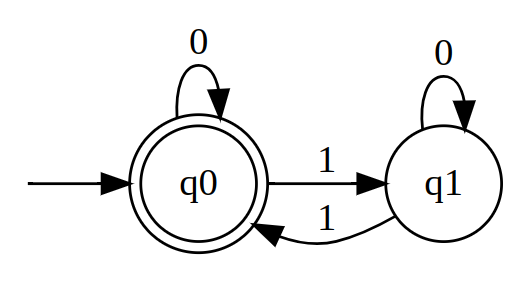
\includegraphics[width=2in]{images/gv/mc02-fa-ex1.png}
\end{frame}

\begin{frame}
  \frametitle{Example 2}

  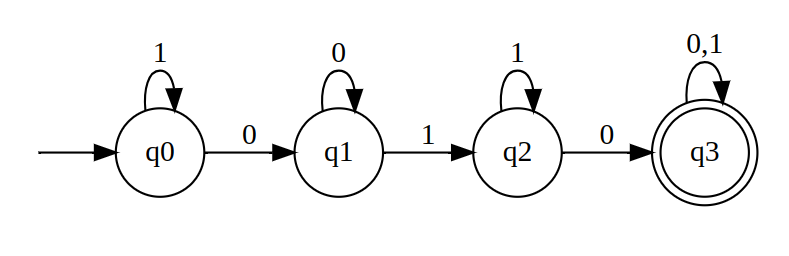
\includegraphics[width=3in]{images/gv/mc02-fa-ex2.png}
\end{frame}

\begin{frame}
  \frametitle{Moves}

  {\bf One step move}: from state $q$ with input symbol $a$, the
  machine changes its state to \pause $\delta(q,a)$.

  {\bf Extension:} from state $q$ with input string $q$, the machine
  changes its state to $\delta^*(q,w)$ defined as

  \pause

  \begin{block}{}
  \[
  \delta^*(q,w) = \left\{
  \begin{array}{ll}
    q & \mbox{if $w=\epsilon$,} \\
    \delta^*(\delta(q,a),x) & \mbox{if $w=ax$.}
  \end{array}
  \right.
  \]
  \end{block}
  
  The signature of $\delta^*$ is $Q\times\Sigma^* \longrightarrow Q$.
\end{frame}

\begin{frame}
  \frametitle{Acceptance}

  For a finite-state machine with starting state $s$ and accepting
  states $A$, it accepts string $w$ iff

  \pause

  \[
  \delta^*(s,w)\in A.
  \]
  
\end{frame}

\begin{frame}[fragile]
  \frametitle{Multiple of 5}

  \begin{columns}
    \begin{column}{0.5\textwidth}
      \pause
\begin{verbatim}
def multiple_of_5(w):
    r = 0
    for i in w:
        r = (2*r + w) % 5
    return r == 0
\end{verbatim}        
    \end{column}
    \begin{column}{0.5\textwidth}
      \pause
      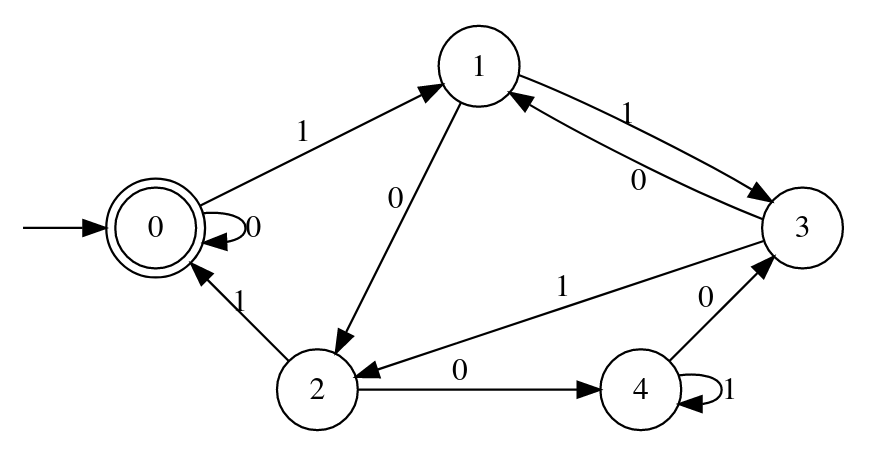
\includegraphics[width=2.5in]{images/gv/mc02-fa-ex3.png}
    \end{column}
  \end{columns}
\end{frame}

\begin{frame}
  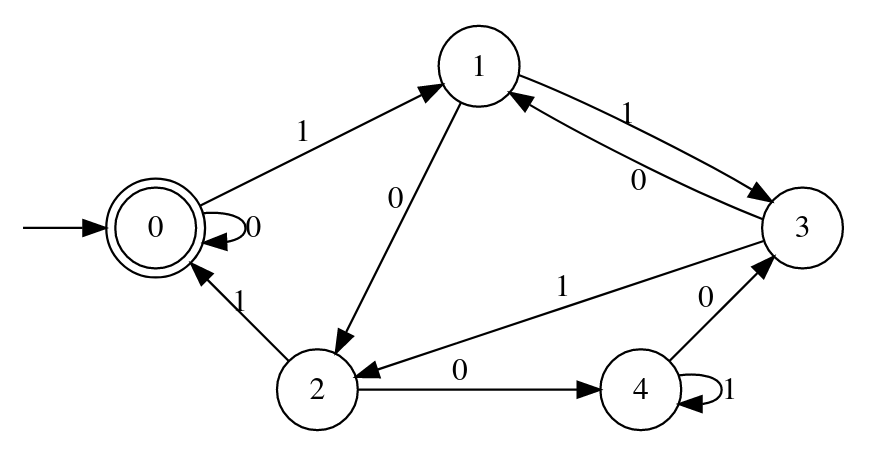
\includegraphics[width=3in]{images/gv/mc02-fa-ex3.png}
\end{frame}

\begin{frame}
  \frametitle{Digital design: Implementation}

\end{frame}

\begin{frame}
  \frametitle{Digital design: Moore and Mealy machines}

  In the digital design class, you will encounter finite-state
  machines as well.  The version we consider in this class is refered
  to as a {\bf Moore machine}.

  In practices, there is another variant of FSM called {\bf Mealy
    machines}, whose outputs depend on input symbols as well.

  \pause

  Formally, they differ in output function.

  \begin{itemize}
  \item Moore machine: $G:Q \longrightarrow [0,1]$
  \item Mealy machine: $G:Q\times \Sigma \longrightarrow [0,1]$
  \end{itemize}
  
\end{frame}

\begin{frame}
  \frametitle{Example: even number of $\cone$'s}
\end{frame}

\begin{frame}
  \frametitle{Example: strings containing $\czero\czero$ as a substring}
\end{frame}

\begin{frame}
  \frametitle{Combining DFAs}

  What if we want to build a DFA that accepts strings with an even
  number of $\cone$'s and containing $\czero\czero$ as a substring?

  \vspace{2in}
\end{frame}

\begin{frame}
  \frametitle{Product construction}
\end{frame}

\begin{frame}
  \frametitle{Product construction (formally)}

  Given a DFA $M_1=(\Sigma,Q_1,\delta_1,s_1,A_1)$ that accepts strings
  from language $L_1$ and $M_2=(\Sigma,Q_2,\delta_2,s_2,A_2)$ that
  accepts strings from language $L_2$, we can construct a DFA
  $M=(\Sigma,Q,\delta,s,A)$ that accepts strings from $L_1\cap L_2$ as
  follows:

  \begin{itemize}
  \item Let $Q=Q_1\times Q_2$, \pause
  \item Let $\delta: (Q_1\times Q_2)\times \Sigma \longrightarrow (Q_1\times Q_2)$ be such that \pause
    \[
    \delta((q_1,q_2),a) = (\delta_1(q_1,a), \delta_2(q_2,a)),
    \]
    \pause
  \item Let $s=(s_1,s_2)$, and \pause
  \item Let $A=A_1\times A_2$.
  \end{itemize}
  
\end{frame}

\begin{frame}

  {\small
    Recall the definition of $\delta^*(q,w)$, i.e., \pause
    \[
    \delta^*(q,w) = \left\{
    \begin{array}{ll}
      q & \mbox{if $w=\epsilon$,} \\
      \delta^*(\delta(q,a),x) & \mbox{if $w=ax$ where $a\in\Sigma$}
    \end{array}
    \right.
    \]
  }
  \pause
  \begin{lemma}
    $\delta^*((q_1,q_2),w) = (\delta_1^*(q_1,w),\delta_2^*(q_2,w))$
    for any string $w$.
  \end{lemma}

  \begin{proof}
    {\small
      We prove by induction.  I.H.: Assume that
      $
      \delta^*((q_1,q_2),x) = (\delta_1^*(q_1,x),\delta_2^*(q_2,x)),
      $
      for any string $x$ such that $|x|<|w|$.
    }
    \vspace{1.2in}
    
  \end{proof}
  
\end{frame}

\begin{frame}

  \frametitle{Correctness}

  From the previous lemma, we have that
  \begin{eqnarray*}
    \delta^*(s,w) &=& \delta^*((s_1,s_2),w) \\ \pause
    &=& (\delta_1^*(s_1,w),\delta_2^*(s_2,w))
  \end{eqnarray*}

  \pause

  Thus, for an input $w$, $M$ would reach the state
  $(\delta_1^*(s_1,w),\delta_2^*(s_2,w))$; it accepts $w$ when
  \[
  (\delta_1^*(s_1,w),\delta_2^*(s_2,w))\in A_1\times A_2.
  \]
  This implies that $M$ accepts $w$ when $\delta_1^*(s_1,w)\in A_1$
  and $\delta_2^*(s_2,w)\in A_2$, i.e., $M$ accepts $w$ iff $M_1$ and
  $M_2$ accept $w$.

  Finally, we conclude that $M$ accepts strings from language $L_1\cap
  L_2$.
  
\end{frame}

\begin{frame}
  \frametitle{Language of a DFA}

  \begin{block}{$L(M)$}
    For a DFA $M$, let $L(M)$ be the set of all strings that $M$
    accepts.  More formally, for $M=(\Sigma,Q,\delta,s,A)$,
    \[
    L(M)=\{w\in\Sigma^* \;|\; \delta^*(s,w)\in A\}.
    \]
    We refer to $L(M)$ as the language of $M$.
  \end{block}
  
\end{frame}

\begin{frame}

  \frametitle{Closure}

  \begin{lemma}
    If $L_1$ and $L_2$ are languages of some DFAs $M_1$ and $M_2$,
    we have that
    \begin{itemize}
    \item there is a DFA $M$ that accepts $L_1\cap L_2$, \pause
    \item there is a DFA $M$ that accepts $L_1\cup L_2$, \pause
    \item there is a DFA $M$ that accepts $L_1\setminus L_2$, \pause
    \item there is a DFA $M$ that accepts $\Sigma^* \setminus L_1$,
    \end{itemize}
  \end{lemma}
  
\end{frame}

\begin{frame}

  \frametitle{Automatic languages\footnote{Taken directly from Erickson's lecture notes}}

  \begin{block}{Definition (for now)}
    A language $L$ is {\color{red}\bf ``automatic''} if there is a DFA $M$
    such that $L(M)=L$.
  \end{block}

  \pause

  \begin{lemma}
    If $L_1$ and $L_2$ are automatic languages over alphabet $\Sigma$,
    then
    \begin{itemize}
    \item $L_1\cap L_2$, \pause
    \item $L_1\cup L_2$, \pause
    \item $L_1\setminus L_2$, and \pause
    \item $\Sigma^* \setminus L_1$,
    \end{itemize}
    are also automatic.
  \end{lemma}

  \pause

  The set of automatic languages is closed under these boolean
  operations.
  
\end{frame}

